\chapter{Efficient Incremental Search}
\label{chap:ibid}

In Chapter~\ref{chap:lazysp},
we introduced the Lazy Shortest Path (LazySP) algorithm,
which addresses domains with expensive edge weight functions
by interleaving the evaluation phase with a sequence of 
search queries using an existing pathfinding algorithm.
Because this inner search is conducted many times,
its efficiency is paramount.

Most approaches for reducing the computational cost of pathfinding
attempt to focus the search on a smaller subset of the graph.
We consider three classes of such techniques
(Figure~\ref{fig:ibid:intro-focus}):

\begin{marginfigure}[5cm]%
   \centering%
   \subfloat[Bidirectional search.]{%
      \centering %
      \includegraphics{build/ibid-intro-focus-bidirectional} %
   }%
   
   \subfloat[Heuristic search.]{%
      \centering %
      \includegraphics{build/ibid-intro-focus-heuristic} %
   }%
   
   \subfloat[Incremental search. \ssnote{hard to follow}]{%
      \centering %
      \includegraphics{build/ibid-intro-focus-incremental} %
   }%
   
   \caption{Illustrations of the three focusing techniques considered
      on a spatial pathfinding problem.}%
   \label{fig:ibid:intro-focus}
\end{marginfigure}

\begin{enumerate}
\item \emph{Bidirectional Search} -- A bidirectional algorithm
   conducts two concurrent searches,
   one from the source vertex $s$,
   and the other from the sink vertex $t$.
   Such searches are well-suited to roadmaps in ambient spaces that
   are high-dimensional \ssnote{how does this translate to number of nodes
   or edges or degree?} and/or have
   obstacles situated close to the source/sink vertices
   \ssnote{hmm, isn't bidirectional Djikstra best when the searches
   meet in the middle, so won't it expand a lot more nodes if sources
   or sinks are harder when compared to both being equally hard?}.
\item \emph{Heuristic Search} -- A heuristic-informed algorithm
   exploits a sink-directed heuristic function over vertices to bias
   exploration in the direction of the sink vertex.
   A strong and admissible such heuristic can drastically speed the
   search, \ssnote{might want to specify exactly how, i.e. expanding
   fewer vertices}
   although the efficacy is reduced for weaker heuristics.
\item \emph{Incremental Search} -- An incremental algorithm
   is applied to a sequence of search queries on a graph whose
   edge weight function changes (partially) between queries.
   \ssnote{isn't this a bit too specific?
   doesn't it also apply to cases where the vertex topology changes?}
   It endeavors to only consider the portion of its data structure
   affected by the changes. \ssnote{might want to say that it's called
   \emph{incremental} because it incrementally updates only the portion
   of the data structure that is relevant for solving the problem.}
\end{enumerate}

The principal contribution of this chapter is IBiD,
an algorithm which combines these three techniques into a single
algorithm
(Table~\ref{tab:ibid:alg-overview}).
While originally motivated for use with LazySP,
IBiD is broadly applicable to incremental search problems.

\paragraph{Chapter outline.}
Finding shortest paths on graphs is a very extensively studied problem.
This chapter begins with a comprehensive review of 
methods which solve shortest path problems by computing
distance functions.
After defining the problem in Section~\ref{subsec:ibid-probdef},
we review distance functions and unidirectional methods
in Section~\ref{sec:ibid:distance-functions}.
Section~\ref{sec:ibid:bidirectional} reviews
bidirectional search methods,
and Section~\ref{sec:ibid:incremental} reviews incremental search.
Section~\ref{sef:ibid:ibid}, introduces IBiD,
an algorithm which combines bidirectional and incremental search.
In Section~\ref{sec:ibid:heuristic},
we review heuristic search methods,
and discuss a heuristic-informed generalization of IBiD.
The chapter concludes with experimental results and implentation notes.

\begin{table}
   \centering
   \begin{tabular}{ccc}
      \toprule
      & Unidirectional & Bidirectional \\
      \midrule
      \addlinespace[0.2em]
      Complete
         & Dijkstra \citep{dijkstra1959anote}
         & Bidirectional Dijkstra \citep{luby1989bidijk} \\
      \addlinespace[-0.2em]
      \emph{(Heuristic)}
         & \emph{A* \citep{hart1968astar}}
         & \emph{Bidirectional A* \citep{ikeda1994betterroutes}} \\
      \addlinespace[0.3em]
      Incremental
         & DynamicSWSF-FP \citep{ramalingam1996dynamicswsffp}
         & {IBiD} \\
      \addlinespace[-0.2em]
      \emph{(Heuristic)}
         & \emph{Lifelong Planning A* \citep{koenig2004lpastar}}
         & \emph{Heuristic IBiD} \\
      \addlinespace[0.2em]
      \bottomrule
   \end{tabular}
   \caption{
      IBiD generalizes both the heuristic-informed
      bidirectional Dijkstra's search \citep{goldberg2005spexternalmemory}
      and DynamicSWSF-FP \citep{ramalingam1996dynamicswsffp}.
      There are a great many algorithms that we could place in each cell;
      we provide only a represetative choice in each.}
   \label{tab:ibid:alg-overview}
\end{table}

\section{Problem Definition}
\label{subsec:ibid-probdef}

The \emph{shortest path problem} on graphs has been extensively
studied over the past six decades.
Consider a directed graph $G = (V,E)$ and accompanying edge weight
function $w : E \rightarrow \mathbb{R}$.
Note that we allow graphs with multiple edges connecting any pair
of vertices,
as well as graphs with edges to and from the same vertex.

The length of a path is equal to the sum of the weights of its
constituent edges.
\marginnote{
The single-pair problem is also called the \emph{two-terminal} or
\emph{point-to-point} problem.}
We consider the \emph{single-pair shortest path} (SPSP) problem,
in which a path of minimal length is sought
between distinct start and destination vertices
$s,t \in V$.
(We can also handle planning problems with multiple
start/goal configurations as an SPSP problem
as described in Section~\ref{subsec:roadmaps:planning-as-pathfinding}.)

Our review is applicable to problems where $w$ is everywhere finite.
The algorithms that we consider do not distinguish between non-existant
and infinite-weight edges,
and so will return that no path exists in the case where shortest
paths contain infinite-weight edges.

\paragraph{An example problem.}
\begin{marginfigure}%
   \centering%
   \begin{tikzpicture}
      \tikzset{>=latex} % arrow heads
      \node[inner sep=0pt,anchor=south west] {%
         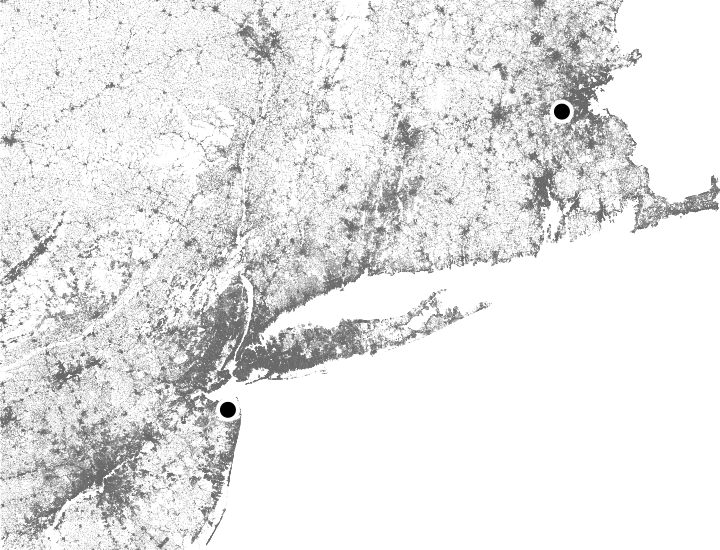
\includegraphics[width=5cm]{figs/incbi-road-ne/singleshot/example-intro.png}};
      \coordinate (s) at (1.75,0.9);
      \coordinate (t) at (3.93,2.8);
      \node (slab) at (2.5,0.6) {$s$};
      \node (tlab) at (4.0,1.5) {$t$};
      \draw[->,thick] (slab) -- (s);
      \draw[->,thick] (tlab) -- (t);
   \end{tikzpicture}%
   \caption{A graph of the Northeast USA from the 9th DIMACS
      Implementation Challenge
      comprises 1,524,453 vertices and 3,868,020 directed edges.
      A shortest path problem from a source $s$ in New Jersey
      to a target $t$ outisde Boston
      will be used as an example.}%
   \label{fig:ibid:example-intro}%
\end{marginfigure}
We will carry forward an illustrative example problem from
the public dataset of the 9th DIMACS Implementation Challenge
\citep{demetrescuetal2006dimacs9}
(Northeast USA)
comprising an approximate road network,
using transit time as the edge weight function
(Figure~\ref{fig:ibid:example-intro}).
In this way,
a shortest path between a pair of start and destination locations
minimizes the total transit time between them.
\ssnote{Might want to provide 1-2 sentence intuition on why
this graph is interesting, and why we chose it for IBID. 
High degree? Nonuniform degree?
Large variation in edge weights?}

\paragraph{Problem Settings.}
The single-pair problem has been extensively studied.
There are techniques that are particular to memory-constrained
settings \citep{kaindl1997biheurreconsidered}
or to settings where pre-computation is available
\citep{goldberg2007pointtopoint}.
While we do not focus on such settings,
the algorithms we propose may be complementary to these techniques.

\section{Review of Pathfinding with Distance Functions}
\label{sec:ibid:distance-functions}

This section contains a unified presentation of unidirectional,
bidirectional, and incremental search stategies
by examining the properties of the distance functions that they
maintain.
These properties and invariants can be established for arbitrary
distance function approximations.
Examination of these properties then informs the development of
algorithms which calculate them,
which we defer to Section~\ref{sef:ibid:ibid}.

While much of this section summaries prior work,
the presentation of the bidirectional termination condition
(Theorem~\ref{thm:ibid-bidir-sound}
in Section~\ref{sec:ibid:bidirectional})
in particular
is formulated to enable the novel theorems
presented in Section~\ref{sef:ibid:ibid}.

\subsection{Shortest Paths via the Source Distance Function}

The pioneering pathfinding algorithms of the late 1950s address
a generalization of the SPSP problem called
the \emph{single-source} problem,
where shortest paths are calculated from the start vertex $s$
to all vertices on the graph.
They proceed by calculating the \emph{source distance function}
$d^* : V \rightarrow \mathbb{R}$,
which gives the length of the shortest path from $s$
to each vertex $v$.
In other words:
\marginnote{Once the distance function $d^*$ is computed,
a shortest path to any target $t$ can be generated trivially
by walking backwards to $s$ guided by $d^*$.}
\begin{equation}
   d^*(v) = \min_{p \in P_{sv}} \mbox{len}(p),
   \label{eqn:ibid-distance-function-global}
\end{equation}
where $P_{sv}$ is the set of all paths from $s$ to $v$.
\ssnote{Have you defined len elsewhere? If so, provide pointer.
Is it meant to be the sum of weights along the path?
\begin{equation}
   d^*(v) = \min_{p \in P_{sv}} \mbox{len}(p) = \min_{p \in P_{sv}} \sum_{e \in p} w(e),
   \label{eqn:ibid-distance-function-global}
\end{equation}
}
Where no paths to $v$ exist,
we take $d^*(v) = \infty$.
Note that $d^*$ is only well-defined on graphs with no negative-length
cycles reachable from $s$.

\begin{marginfigure}%
   \centering%
   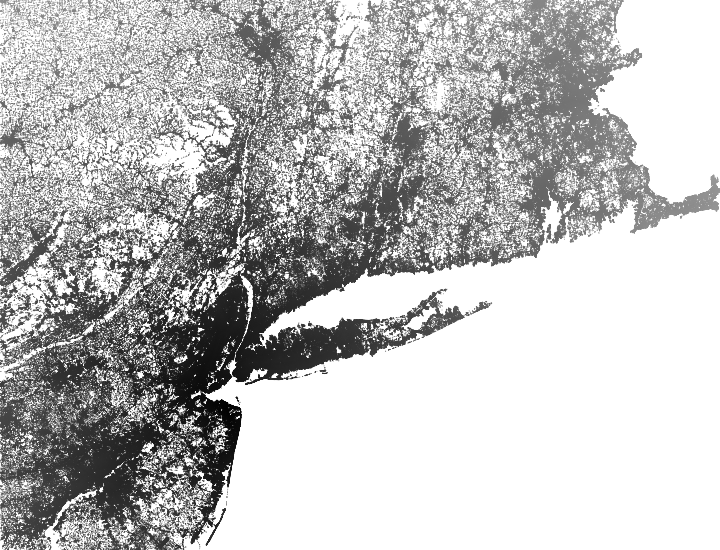
\includegraphics[width=5cm]{figs/incbi-road-ne/singleshot/example-dijkstraall.png}%
   \caption{The distance function from the source vertex.}%
   \label{fig:ibid:example-distance-all}%
\end{marginfigure}

Importantly, $d^*$ can also be characterized locally by
\begin{equation}
   d^*(v) = 
   \left\{ \begin{array}{cl}
      0 & \mbox{if } v = s \\
      \displaystyle\min_{u \in \mbox{\scriptsize Pred}(v)} d^*(u) + w(e_{uv}) & \mbox{otherwise,} \\
   \end{array} \right.
   \label{eqn:distance-function-char}
\end{equation}
where $\mbox{Pred}(v)$ yeilds the predecessor vertices of $v$,
and a vertex $v \neq s$ with no predecessors takes $d^*(v) = \infty$.
\marginnote{Note that
while the distance function $d^*$ necessarily satisfies
the equations (\ref{eqn:distance-function-char}),
they are not generally a sufficint condition;
if a reachable cycle of zero length exists,
(\ref{eqn:distance-function-char}) will not have a unique solution.}
The distance function is akin to the \emph{value function}
in more general decision problems addressed by dynamic programming.
The equations (\ref{eqn:distance-function-char})
are the \emph{Bellman equations} \citep{bellman1958routing},
which rely on the principle of optimality.
This characterization also follows implicitly from early results for
the all-pairs problem
\citep{shimbel1955communicationnets, beckmann1955transportation}.
Note that while (\ref{eqn:distance-function-char})
is a necessary condition of $d^*$,
it is not sufficient in general.
In particular,
if $w$ has cycles of length zero,
then even though $d^*$ is well-defined,
(\ref{eqn:distance-function-char}) admits an infinite number
of incorrect solutions for $d$.

\paragraph{Reconstructing a Shortest Path from the Distance Function}
Calculating the source distance function is only useful for solving
the SPSP problem if it can be used to efficiently determine
a shortest path.
We can show that such a path can be reconstructed by starting at
the destination $t$ and progressively prepending the predecessor
edge $e_{uv}$ (and vertex $u$)
which locally minimizes $d^*(u) + w(e_{uv})$.
Any path constructed in this way is guaranteed to be a shortest path,
and this process is gauranteed to terminate if the graph
contains no zero-length cycles.

\subsection{Approximating $d^*$ via Tensioned Estimates}
\label{subsec:ibid-tension}

How can we compute $d^*$ efficently over the graph?
Consider an approximation function $d$
which satisfies the following four properties:%
\begin{subequations}%
   \begin{eqnarray}
      & d^*(v) \leq d(v) & \forall v
         \label{eqn:ibid-relaxation-props-nounder} \\
      & d(v) = 0 & v = s
         \label{eqn:ibid-relaxation-props-ds0} \\
      & \displaystyle\min_{u \in \mbox{\scriptsize Pred}(v)}
         d(u) + w(e_{uv}) \leq d(v)
         & v \neq s
         \label{eqn:ibid-relaxation-props-nottoogood} \\
      & d(u) + w(e_{uv}) \geq d(v) & \forall e_{uv}
         \label{eqn:ibid-relaxation-props-tens}
   \end{eqnarray}%
   \label{eqn:ibid-relaxation-props}%
\end{subequations}%
Conditions (\ref{eqn:ibid-relaxation-props-ds0} --
\ref{eqn:ibid-relaxation-props-tens})
follow directly from the local characterization
(\ref{eqn:distance-function-char});
in particular,
the case where $v \neq s$ has been split into the two
equivalent inequalities (\ref{eqn:ibid-relaxation-props-nottoogood})
and (\ref{eqn:ibid-relaxation-props-tens}).
In contrast,
for now we take the global inequality
(\ref{eqn:ibid-relaxation-props-nounder}) on faith;
we will later revisit the implications of relying on this assumption.

We can show that any estimate $d$ satisfying these properties
is the unique distance function $d^*$
via Theorem~\ref{thm:ibid-relaxation-notension}.

\begin{theorem}
\marginnote{Proofs for all theorems in this chapter are located in
Appendix~\ref{chap:appendix-ibid-proofs}.}
If $d: V \rightarrow \mathbb{R}$
satisfies (\ref{eqn:ibid-relaxation-props}),
then $d = d^*$.
\label{thm:ibid-relaxation-notension}
\end{theorem}

The principal method for arriving at an approximation
which satisfies (\ref{eqn:ibid-relaxation-props})
is via \emph{tensioned estimates}.
Consider an arbitrary approximation $d$ which satisfies only
(\ref{eqn:ibid-relaxation-props-nounder} --
\ref{eqn:ibid-relaxation-props-nottoogood}),
and consider the following edge labeling:
\begin{equation}
   \mbox{edge } e_{uv} \mbox{ is \emph{tensioned}}
   \;\;\mbox{iff}\;\;
   d(u) + w(e_{uv}) < d(v).
   \label{eqn:ibid-relaxation-tensioned}
\end{equation}
Tensioned edges are therefore those that violate
(\ref{eqn:ibid-relaxation-props-tens}).
A restatement of Theorem~\ref{thm:ibid-relaxation-notension}
is that an approximation $d$
satisfying (\ref{eqn:ibid-relaxation-props-nounder} --
\ref{eqn:ibid-relaxation-props-nottoogood})
with no tensioned edges is everywhere correct.

\paragraph{Edge Relaxation.}
How can we arrive at an approximation
satisfying Theorem~\ref{thm:ibid-relaxation-notension}?
The principal technique treats the properties
(\ref{eqn:ibid-relaxation-props-nounder} --
\ref{eqn:ibid-relaxation-props-nottoogood}) as invariants.
An initial approximation $d$ is chosen for which the invariants
trivially hold,
such as $d(v) = \infty \;\forall v \neq s$,
which will generally have many edges in tension.
The tensioned approximation $d$ is then iteratively improved
via \emph{edge relaxation}
as described by Ford \citep{ford1955networkflowtheory},
wherein a tensioned edge $e_{uv}$ is selected and relaxed
by setting $d(v) \leftarrow d(u) + w(e_{uv})$.
It can be shown that applying this process arbitrarily
maintains the invariants.

It can be further shown that for a finite graph,
the number of edge relaxations needed is also finite.
The well-known Bellman-Ford method
\citep{shimbel1955communicationnets, bellman1958routing,
moore1959spmaze}
cycles through all edges repeatedly,
relaxing all tensioned edges found
(at most $|V|-1$ repetitions are sufficient for convergence).
Note that this does not place any requirements on $w$
(other than that $d^*$ must exist, so there must not be
any negative-length cycles reachable from $s$).

\paragraph{Approximation Soundness.}
The need for multiple cycles of Bellman-Ford stems from the fact
that each edge may need to be relaxed several times.
This occurrs because relaxing an edge changes the
$d$-value of the target vertex,
which may newly tension downstream edges
(see Figure~\ref{fig:ibid:bellman-ford-repetitions}).

\begin{marginfigure}
   \centering
   \begin{tikzpicture}
      \tikzset{>=latex} % arrow heads

      \begin{scope}[shift={(0,0)}]
         \node[fill=black,circle,inner sep=1.2pt] (a) at (0,0) {};
         \node[fill=black,circle,inner sep=1.2pt] (b) at (1.5,0) {};
         \node[fill=black,circle,inner sep=1.2pt] (c) at (3.0,0) {};
         \draw[->,densely dashed] (a) -- (b) node[midway,fill=white,circle,inner sep=1pt] {1};
         \draw[->,densely dashed] (b) -- (c) node[midway,fill=white,circle,inner sep=1pt] {1};
         
         \node[above=-0.00cm of a] {$a$};
         \node[above=-0.00cm of b] {$b$};
         \node[above=-0.00cm of c] {$c$};

         \node[below=0.05cm of a] {$d=0$};
         \node[below=0.05cm of b] {$d=2$};
         \node[below=0.05cm of c] {$d=4$};
      \end{scope}

      \begin{scope}[shift={(0,-1)}]
         \node[fill=black,circle,inner sep=1.2pt] (a) at (0,0) {};
         \node[fill=black,circle,inner sep=1.2pt] (b) at (1.5,0) {};
         \node[fill=black,circle,inner sep=1.2pt] (c) at (3.0,0) {};
         \draw[->,densely dashed] (a) -- (b) node[midway,fill=white,circle,inner sep=1pt] {1};
         \draw[line width=0.10cm,black!10] (b) -- (c) node[midway,fill=white,circle,inner sep=1pt] {1};
         \draw[->] (b) -- (c) node[midway,fill=white,circle,inner sep=1pt] {1};

         \node[below=0.05cm of a] {$d=0$};
         \node[below=0.05cm of b] {$d=2$};
         \node[below=0.05cm of c] {$d=3$};
      \end{scope}

      \begin{scope}[shift={(0,-2)}]
         \node[fill=black,circle,inner sep=1.2pt] (a) at (0,0) {};
         \node[fill=black,circle,inner sep=1.2pt] (b) at (1.5,0) {};
         \node[fill=black,circle,inner sep=1.2pt] (c) at (3.0,0) {};
         \draw[line width=0.10cm,black!10] (a) -- (b) node[midway,fill=white,circle,inner sep=1pt] {1};
         \draw[->] (a) -- (b) node[midway,fill=white,circle,inner sep=1pt] {1};
         \draw[->,densely dashed] (b) -- (c) node[midway,fill=white,circle,inner sep=1pt] {1};
         
         \node[below=0.05cm of a] {$d=0$};
         \node[below=0.05cm of b] {$d=1$};
         \node[below=0.05cm of c] {$d=3$};
      \end{scope}

      \begin{scope}[shift={(0,-3)}]
         \node[fill=black,circle,inner sep=1.2pt] (a) at (0,0) {};
         \node[fill=black,circle,inner sep=1.2pt] (b) at (1.5,0) {};
         \node[fill=black,circle,inner sep=1.2pt] (c) at (3.0,0) {};
         \draw[->] (a) -- (b) node[midway,fill=white,circle,inner sep=1pt] {1};
         \draw[line width=0.10cm,black!10] (b) -- (c) node[midway,fill=white,circle,inner sep=1pt] {1};
         \draw[->] (b) -- (c) node[midway,fill=white,circle,inner sep=1pt] {1};
         
         \node[below=0.05cm of a] {$d=0$};
         \node[below=0.05cm of b] {$d=1$};
         \node[below=0.05cm of c] {$d=2$};
      \end{scope}
      
   \end{tikzpicture}
   \caption{Ordering problems.
      Consider the vertices $a \rightarrow b \rightarrow c$,
      with edges $e_{ab}$ and $e_{bc}$ both in tension;
      if $e_{bc}$ is relaxed before $e_{ab}$,
      then $e_{bc}$ will need to be relaxed a second time.}
   \label{fig:ibid:bellman-ford-repetitions}
\end{marginfigure}

We can exploit our intution to order relaxations from start to destination
in the special case where $w \geq 0$
(note that this requirement is stronger than requiring no reachable
negative-length cycles).
We can then show that our approximation $d$
is \emph{sound} for a subset of vertices
as described by Theorem~\ref{thm:ibid-relaxation-sound}.

\begin{marginfigure}
   \centering
   \includegraphics{build/ibid-dijkstra-trust}
   \caption{Tensioned edge trust region
      for $w \geq 0$.
      Contours are of the current estimate $d$.
      Currently tensioned edges are bold and dotted.}
\end{marginfigure}

\begin{theorem}
Consider $d: V \rightarrow \mathbb{R}$
satisfying (\ref{eqn:ibid-relaxation-props-nounder} --
\ref{eqn:ibid-relaxation-props-nottoogood}),
and let $D$ be the smallest value $d(u)$
among all tensioned edges $e_{uv}$
(or $\infty$ if no such edges exist).
If $w \geq 0$,
any vertex $x$ with $d(x) \leq D$
has $d(x) = d^*(x)$.
\label{thm:ibid-relaxation-sound}
\end{theorem}
As a result,
a given value $k$ creates a region of vertices
with values $d(x) \leq D$ that are known to be
accurate.
This confers two distinct advantages when designing an algorithm:
an efficient relaxation ordering,
and an early termination condition for single-pair problems.

\paragraph{Efficient Relaxation Ordering.}
Therefore,
all tensioned edges $e_{uv}$ with $d(u) = D$
(of which there must be at least one if any edges are tensioned)
can be relaxed immediately,
and will never be retensioned.
This is exactly the order imposed by the OPEN list in Dijkstra's
algorithm \citep{dijkstra1959anote}.

\begin{marginfigure}%
   \centering%
   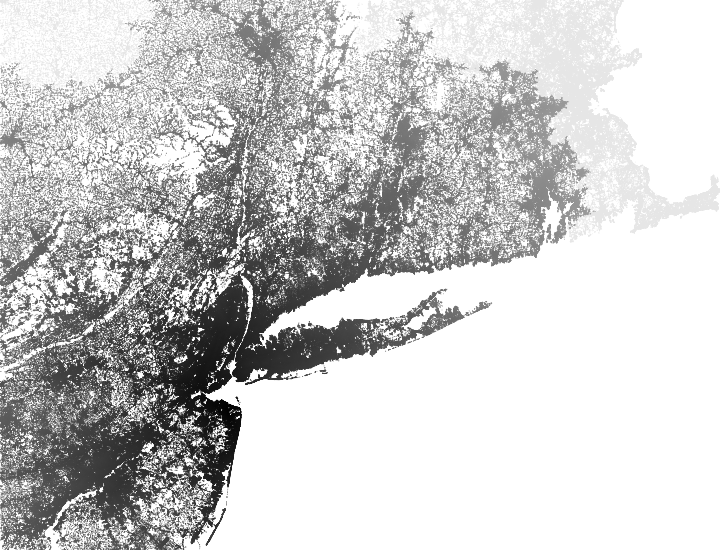
\includegraphics[width=5cm]{figs/incbi-road-ne/singleshot/example-dijkstra.png}%
   \caption{Dijkstra's algorithm computes the start distance function
      $d^*$ to solve the example shortest path problem.
      Darker vertices have smaller $d$-values.
      The algorithm stops upon reaching the target vertex $t$
      after expanding 1,290,820 vertices.}%
   \label{fig:ibid:example-distance}%
\end{marginfigure}

\paragraph{Early Termination.}
The soundness result shows that once the destination
vertex $t$ satisfies $d(t) \leq D$,
it has the correct start distance.
Since we are only interested in reconstructing a shortest path to $t$,
we are interested in terminating computation of the distance
function as early as possible.
However,
Theorem~\ref{thm:ibid-relaxation-sound} by itself is insufficient
to demonstrate that such a shortest path can be reconstructed.
This requres a proof of Theorem~\ref{thm:ibid-relaxation-reconstruct}.

\begin{theorem}
Consider $d: V \rightarrow \mathbb{R}$
satisfying (\ref{eqn:ibid-relaxation-props-nounder} --
\ref{eqn:ibid-relaxation-props-nottoogood}),
and let $D$ be the smallest value $d(u)$
among all tensioned edges $e_{uv}$
(or $\infty$ if no such edges exist).
If $w \geq 0$,
for any vertex $x$ with $d(x) \leq D$,
a path reconstructed backwards from $x$ by iteratively selecting a
predecessor minimizing $d(u) + w(e_{uv})$ until $s$ is reached
is a shortest path from $s$ to $x$ of length $d^*(x)$.
\label{thm:ibid-relaxation-reconstruct}
\end{theorem}

%Unfortunately the edge cases for completeness are less strong
%than for soundness.
%See the example in Figure~\ref{fig:ibid:relaxation-completeness-issue}.
%\cdnote{Add note about how in the special case where $d$ is initialized
%to $\infty$ and all $d$-values are thereafter reduced via edge
%relaxations,
%this completeness result also extends to the case of
%$w \geq 0$ and $d^*(x) \leq d'$.
%But this result isn't applicable to incremental settings as we'll
%discuss in Section~\ref{sec:ibid:incremental}.}

%\begin{marginfigure}
%   \centering
%   \begin{tikzpicture}
%      \tikzset{>=latex} % arrow heads
%      \node[fill=black,circle,inner sep=1.2pt] (s) at (0,0) {};
%      \node[fill=black,circle,inner sep=1.2pt] (a) at (1.5,0) {};
%      \node[fill=black,circle,inner sep=1.2pt] (b) at (1.5,1.2) {};
%      \node[fill=black,circle,inner sep=1.2pt] (x) at (3.0,0) {};
%      \draw[->,densely dashed] (s) -- (a) node[midway,fill=white,circle,inner sep=1pt] {0};
%      \draw[->] (a) -- (x) node[midway,fill=white,circle,inner sep=1pt] {0};
%      \draw[->] (s) -- (b) node[midway,fill=white,circle,inner sep=1pt] {1};
%      \draw[->] (b) -- (x) node[midway,fill=white,circle,inner sep=1pt] {1};
%
%      \node[above=0.05cm of s] {$s$};
%      \node[above=0.05cm of a] {$a$};
%      \node[below=0.05cm of b] {$b$};
%      \node[above=0.05cm of x] {$x$};
%
%      \node[below=0.05cm of s] {$d=0$};
%      \node[below=0.05cm of a] {$d=3$};
%      \node[above=0.35cm of b] {$d=1$};
%      \node[below=0.05cm of x] {$d=0$};
%
%      \node[below=0.35cm of s] {$d^*=0$};
%      \node[below=0.35cm of a] {$d^*=0$};
%      \node[above=0.05cm of b] {$d^*=1$};
%      \node[below=0.35cm of x] {$d^*=0$};
%   \end{tikzpicture}
%   \caption{Problem case for pathfinding with distance functions.
%      Here, $d$ satisfied a and c, with edge $e_{sa}$ tensioned,
%      and $d' = 0$.
%      While the approximation $d$ is \emph{sound} at $x$
%      ($d(x)$ is correct),
%      reconstructing a shortest path requires \emph{completeness}.}
%   \label{fig:ibid:relaxation-completeness-issue}
%\end{marginfigure}

\subsection{Bidirectional Search}
\label{sec:ibid:bidirectional}

A prominent technique for minimizing pathfinding computation for
single-pair problems
is bidirectional search.
In a bidirectional algorithm,
the distance $d_t$ to the target is calculated in a growing region
around the target vertex $t$
concurrently with the conventional source distance $d_s$ around $s$
(Figure~\ref{fig:ibid:example-bidirectional}).
Loosely speaking,
the search can terminate with a shortest path
once the two regions intersect.
The savings relative to a unidirectional search grow with the problem's
branching factor.
For roadmap graphs embedded in an ambient space,
this branching factor can be linear or exponential in the space's
dimension.
\begin{marginfigure}%
   \centering%
   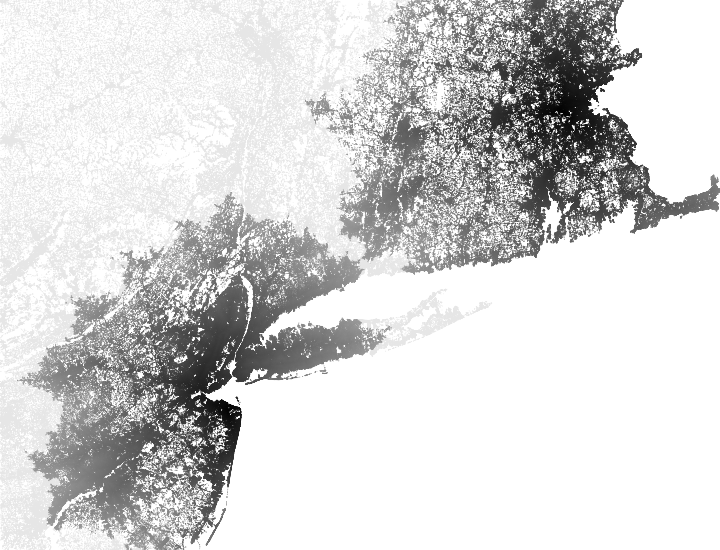
\includegraphics[width=5cm]{figs/incbi-road-ne/singleshot/example-bidijkstra.png}%
   \caption{The bidirectional Dijkatra's algorithm
      computes $d_s$ around the source vertex
      and $d_t$ around the target vertex.
      Darker vertices have smaller $d$-values in their respective
      regions.
      The algorithm terminates after expanding a total of
      1,178,200 vertices using distance to balance expansions.}%
   \label{fig:ibid:example-bidirectional}%
\end{marginfigure}

The first bidirectional algorithm
was proposed by Dantzig \citep{dantzig1963linearprogramming},
and the first precisely described algorithm was presented by
Nicholson \citep{nicholson1966shortest}.
%Implementation of a sound and efficient algorithm
%turns on two important questions:
%(a) when and how to terminate with a shortest path,
%and (b) how to balance expansions from the two directions of the
%search.
Implementation of a sound and efficient algorithm
turns on when and how to terminate with a shortest path.

\paragraph{A Correct Termination Condition.}
%\label{sec:ibid:bidirectional-termination}
What happens upon an encounter between the forward and reverse searches?
Consider running each search until the first vertex is found
that satisfies Theorem~\ref{thm:ibid-relaxation-sound} in both
directions
(that is, the first vertex $x$ for which
$d_s(x) \leq D_s$ and $d_t(x) \leq D_t$).
While Theorem~\ref{thm:ibid-relaxation-sound} correctly demonstrates
that the values $d_s(x)$ and $d_t(x)$ are correct
(and Theorem~\ref{thm:ibid-relaxation-reconstruct} similarly
demonstrates that a shortest path can be reconstructed from $s$ to $x$
and also from $x$ to $t$),
this is not sufficient to demonstrate that the shortest path
actually passes through $x$.
See Figure~\ref{fig:ibid:bidirectional-termination-issue} for a
counter-example that illustrates this point.

\begin{marginfigure}
   \centering
   \begin{tikzpicture}
      \tikzset{>=latex} % arrow heads
      \node[fill=black,circle,inner sep=1.2pt] (s) at (0,0) {};
      \node[fill=black,circle,inner sep=1.2pt] (a) at (1.5,0) {};
      \node[fill=black,circle,inner sep=1.2pt] (b) at (3.0,0) {};
      \node[fill=black,circle,inner sep=1.2pt] (t) at (4.5,0) {};
      \node[fill=black,circle,inner sep=1.2pt] (c) at (2.25,0.8) {};
      \draw[->] (s) -- (a) node[midway,fill=white,circle,inner sep=1pt] {3};
      \draw[->] (a) -- (b) node[midway,fill=white,circle,inner sep=1pt] {3};
      \draw[->] (b) -- (t) node[midway,fill=white,circle,inner sep=1pt] {3};
      \draw[->] (a) -- (c) node[midway,fill=white,circle,inner sep=1pt] {2};
      \draw[->] (c) -- (b) node[midway,fill=white,circle,inner sep=1pt] {2};
      \node[below=0.05cm of s] {$s$};
      \node[below=0.05cm of a] {$a$};
      \node[below=0.05cm of b] {$b$};
      \node[below=0.05cm of t] {$t$};
      \node[above=0.05cm of c] {$c$};
   \end{tikzpicture}
   \caption{Simple illustration of a problem case for terminating
      a bidirectional search.
      With a balanced distance criterion,
      $c$ will be the first vertex expanded in both directions,
      but it does not lie on the shortest path.}
   \label{fig:ibid:bidirectional-termination-issue}
\end{marginfigure}

Importantly, is nececessary to consider the \emph{edges} connecting
the two distance function approximations.
A correct termination condition is surprisingly subtle,%
\marginnote{There were early incorrect attempts at a sound
termination condition
\citep{berge1965programminggamestransportation}.}
with several correct variations proposed
\citep{nicholson1966shortest, dreyfus1969appraisalsp,
pohl1969bidirectional, goldberg2005spexternalmemory}.
What is necessary is a bidirectional equivalent to the 
completeness-based termination condition
from Theorem~\ref{thm:ibid-relaxation-reconstruct}.

Suppose $d_s$ and $d_t$ are approximations to $d^*_s$ and $d_t^*$,
respectively,
with each satisfying (\ref{eqn:ibid-relaxation-props}).
Let $D_s$ be the minimum $u$-value among all tensioned edges in $d_s$
(and likewise for $d_t$).
Then we can establish the following proof of a correct termination
condition:

\begin{theorem}
Define $E_{\ms{conn}}$ as the set of all edges $e_{uv}$ such that
$d_s(u) \leq D_s$ and $d_t(v) \leq D_t$,
and define $\ell_e$ s.t. $\ell_e(e_{uv}) = d_s(u) + w(e_{uv}) + d_t(v)$.
If $w \geq 0$,
$s \neq t$,
$E_{\ms{conn}}$ is non-empty,
and $e^*_{uv}$ minimizes $\ell_e$
among $E_{\ms{conn}}$ with $\ell_e(e^*_{uv}) \leq D_s + D_t$,
then $\ell_e(e^*_{uv})$ is the length of the shortest path,
and $e^*_{uv}$ lies on one such path.
\label{thm:ibid-bidir-sound}
\end{theorem}

\paragraph{Designing an Efficient Bidirectional Algorithm.}
In the case where the approximations $d_s$ and $d_t$ are improved
via edge relaxation,
since $w \geq 0$,
by Theorem~\ref{thm:ibid-relaxation-sound}
once an edge $e_{uv}$ becomes included in
$E_{\ms{conn}}$,
its length value $\ell_e(e_{uv})$ will not change.
Therefore,
it is sufficient for a relaxation algorithm to consider only edges
newly added to $E_{\ms{conn}}$ at each iteration,
and keep track of the best edge $e^*_{uv}$
with its value $\ell_e(e^*_{uv})$ found so far.
Note also that Theorem~\ref{thm:ibid-relaxation-reconstruct}
allows a shortest path to be constructed from $e^*_{uv}$
buy walking backwards from $u$ to $s$,
and forwards from $v$ to $t$.

%\subsection{Balancing Directions}
%The general bidirectional algorithm leaves open the strategy
%used to balance the progression of the two search directions.
%Options based on alternating \citep{dantzig1963linearprogramming},
%or selecting the direction with the smaller {\sc Open} distance
%\citep{nicholson1966shortest}
%or {\sc Open} (and finite) set cardinality
%\citep{pohl1969bidirectional}
%have been proposed.
%Note that while some literature asserts that
%these can be interleaved arbitrarily,
%termination of the algorithm requires that each direction
%be expanded at least once.
%Our example problems use the balanced distance criterion.

\subsection{Incremental Search for Dynamic Problems}
\label{sec:ibid:incremental}

The shortest path on a graph is of course intimately tied to
the edge weight function $w$.
If the weight function changes from $w$ to $w'$,
a shortest path $p$ w.r.t. $w$
will generally no longer be a shortest path w.r.t. $w'$,
even if changes are small and localized.
For example,
if the weight of edge on $p$ increases,
or if the weight of some edge not on $p$ decreases,
then some other path $p'$ may become shorter than $p$.
The dynamic shortest-path problem considers finding a shortest path
for each of a sequence of input edge weight functions,
and algorithms have been proposed to address the dynamic problem.

\cdnote{
A review is here: \citep{eppstein1999dynamic},
\citep{demetrescu2010dynamic}.
Also how about this: \citep{frigioni2000dynamicsp}.
Also add forward pointer to heuristic stuff.}

\begin{marginfigure}%
   \centering%
   \subfloat[Initial episode]{%
      \centering%
      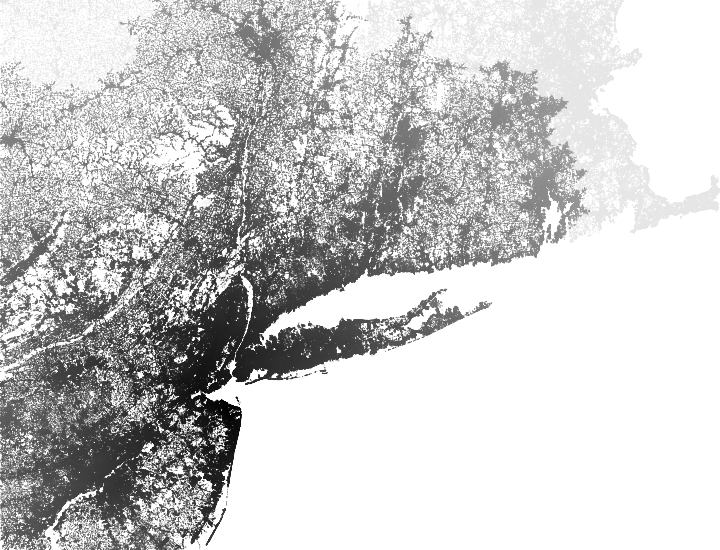
\includegraphics[width=5cm]{figs/incbi-road-ne/singleshot/example-incuni-0.png}%
   }
   
   \subfloat[Subsequent episode]{%
      \centering%
      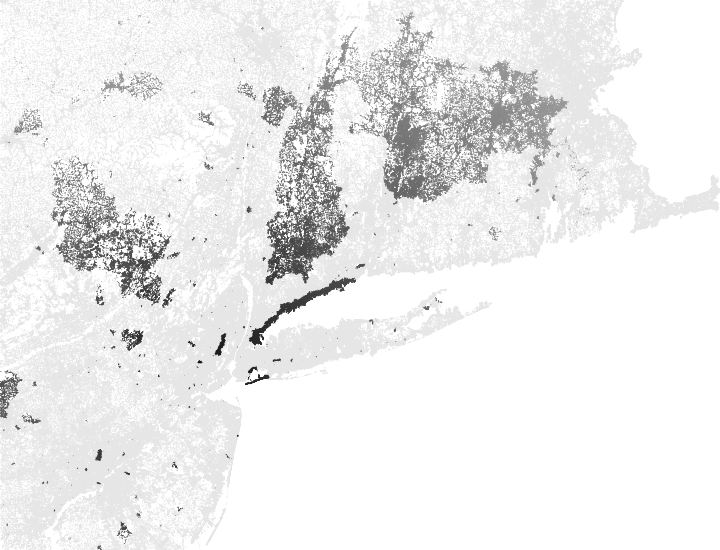
\includegraphics[width=5cm]{figs/incbi-road-ne/singleshot/example-incuni-1.png}%
   }%
   \caption{Initial episode: 1,287,897 expansions.
      Subsequent episode: 391,122 expansions.}%
   %\label{fig:ibid:example-bidirectional}%
\end{marginfigure}

\paragraph{Problem Definition.}
Consider a directed graph $G = (V,E)$ as described in
Section~\ref{subsec:ibid-probdef}.
Consider a sequence of pathfinding episodes
with different edge weight functions $w^{(1)}, w^{(2)}, \dots$
with $w^{(i)} : E \rightarrow \mathbb{R}$.
The dynamic single-pair shortest-path (SPSP) problem
entails finding shortest paths $p^{(1)}, p^{(2)}, \dots$
between fixed start and destination vertices $s,t \in V$
for each episode.

\paragraph{Approches to the Dynamic Problem.}
The simplest class of solutions to the dynamic SPSP problem
entails running a conventional SPSP algorithm to compute a solution
path for episode in turn.
Consider, for example, applying the edge relaxation approach
from Section~\ref{subsec:ibid-tension}
to compute the start distance function $d_s^{(i)}$ from scratch
for each episode's edge weight function $w^{(i)}$.

Investigating this approach more closely reveals an opportunity for
a more efficient algorithm.
If the changes in the weight function between each episode affect
only a subset of the edges,
then it is often the case that the value of the distance function
computed does not change for a large fraction of the vertices in the
graph.
In the face of a change in weight function
$w^{(i)} \rightarrow w^{(i+1)}$,
it is the objective of an \emph{incremental} approach
to adapt a previously computed estimate $d_s^{(i)}$
to a new one $d_s^{(i+1)}$ with a minimal amount of additional
computation.

\paragraph{Inapplicability of the Tensioned Estimates Approach.}
The tensioned estimates approach of Section~\ref{subsec:ibid-tension}
made use of two clever devices to allow its approximation $d$ to be
iteratively improved to the true distance function $d^*$.
First, it relied on a global invariant
(\ref{eqn:ibid-relaxation-props-nounder})
to ensure that the approximation was never under-consistent.
Second, it relied on a decomposition of the local characterization
(\ref{eqn:distance-function-char})
into two inequalities
(\ref{eqn:ibid-relaxation-props-nottoogood})
and (\ref{eqn:ibid-relaxation-props-tens}),
the former treated as a second invariant,
and the latter represented not as a constraint but as a labeling
of tensioned edges to be iteratively relaxed.

Unfortunately,
the incremental setting precludes this approach.
Consider a new episode in which the estimate $d^{(i+1)}$
is initialized with the preceeding estimate $d^{(i)}$.
Since the weight function $w^{(i+1)}$ has changed,
there is no guarantee that either of the invariants
(\ref{eqn:ibid-relaxation-props-nounder})
or (\ref{eqn:ibid-relaxation-props-nottoogood}) still hold.
In particular,
if edge weights increase,
it is common for one or both invariants to be violated,
and we can no longer rely on Theorems~\ref{thm:ibid-relaxation-sound}
or~\ref{thm:ibid-relaxation-reconstruct} to generate sound
shortest paths.

\paragraph{A New Approach.}
The key idea underlying the incremental approach,
and the DynamicSWSF-FP \citep{ramalingam1996dynamicswsffp} algorithm,
is to restate the local characterization (\ref{eqn:distance-function-char})
in a different way.
In particular:
\begin{subequations}%
   \begin{eqnarray}
      & r(v) = 
         \left\{ \begin{array}{cl}
            0 & \mbox{if } v = s \\
            \displaystyle\min_{u \in \mbox{\scriptsize Pred}(v)} d(u) + w(e_{uv}) & \mbox{otherwise} \\
         \end{array} \right.
         & \label{eqn:ibid-inc-props-rvalue} \\
      & d(v) = r(v)
         & \label{eqn:ibid-inc-props-consistent}
   \end{eqnarray}%
   \label{eqn:ibid-inc-props}%
\end{subequations}%
(Here, $r(v)$ represents the ``right-hand side'' of
the local characterization).
It is easy to see how (\ref{eqn:ibid-inc-props}) taken together
directly implies (\ref{eqn:distance-function-char}).
The motivation behind this decomposition is that the former
(\ref{eqn:ibid-inc-props-rvalue}) can be held as an invariant,
while the latter (\ref{eqn:ibid-inc-props-consistent})
can be established iteratively.
Prior work adopts the following labeling for each vertex $v$:
if $d(v) = r(v)$, the vertex is \emph{consistent},
whereas inconsistent vertices are either
\emph{under-consistent} if $d(v) < r(v)$
or \emph{over-consistent} if $d(v) > r(v)$.

Importantly,
the inapplicability of the global invariant
(\ref{eqn:ibid-relaxation-props-nounder}) between episodes
has implications on the class of weight functions that can be solved
by the incremental approach.
In particular,
when applied to weight functions with cycles of zero length
(for which $d^*$ is well-defined),
there is no guarantee that a distance function $d$
which satisfies (\ref{eqn:ibid-inc-props-consistent})
matches $d^*$.
We therefore restrict the class of weight functions considered
to those with only positive length cycles.

\cdnote{TODO: show that the algorithm terminates as long as there
are no cycles with non-positive length.
Lyaponov function argument?}

\paragraph{Approximation Soundness.}
In Section~\ref{subsec:ibid-tension},
we showed that in cases with $w \geq 0$,
the minimal value $k$ defines a trust region that can be used both
to order edge relaxations as well as inform a termination condition
after which a correct path can be reconstructed.
We can develop a similar argument about the soundness of an
approximation in the dynamic case.
In particular,
given an arbitrary estimate $d$
(and the corresponding function $r$ as defined by
(\ref{eqn:ibid-inc-props-rvalue}),
this argument makes use of a third function $k$ defined as:
\begin{equation}
   k(v) = \min\left[ d(v), r(v) \right].
\end{equation}
%If we define $V_{\ms{incons}}$ as the set of inconsistent vertices
%(that is, with $d(v) \neq r(v)$,
%then we define the value $k_{\ms{min}}$ as:
%\begin{equation}
%   k_{\ms{min}} = \displaystyle\min_{v \in V_{\ms{incons}}} \left[ k(v) \right]
%\end{equation}
We can then establish the following central soundness result
for incremental search:

\begin{theorem}
Consider $d: V \rightarrow \mathbb{R}$,
with $r$ satisfying (\ref{eqn:ibid-inc-props-rvalue}),
and let $K$ be the smallest value $k(v)$
among all inconsistent vertices
(or $\infty$ if no such vertices exist).
If $w > 0$,
any consistent vertex $x$ with $d(x) \leq K$
has $d(x) = d^*(x)$.
Further,
walking backwards from $x$ choosing predecessors that minimize
$d(u) + w(e_{uv})$ terminates at $s$ with a shortest path
of length $d^*(x)$.
\label{thm:ibid-dynamicswsffp-sound}
\end{theorem}

This theorem enables the same two efficiency advantages as in
the relaxation approach, in the case where $w > 0$.
It provides that a vertex rendered consistent during an iteration
(by setting $d(x) \leftarrow r(x)$) with $d(x) \leq K$
has the correct value and will never be revisited.
It also enables an algorithm to terminate early
once the destination vertex $t$ becomes consistent,
as exploited by the Lifelong Planning A* algorithm
\citep{koenig2004lpastar}.

\subsection{Algorithm Design}

\cdnote{I still need to write this part!
Talk about queues!}

% I don't need this anymore, subsumed in soundness result!
%\paragraph{Approximation Completeness.}
%
%For bidirectional search,
%it's also necessary to be able to prove that you have found
%all vertices within a certain distance of the start.
%Basically, this is a completeness proof --
%if a distance exists below a certain value,
%we will have found it.
%This is completeness of the approximation,
%not of an algorithm per se.
%
%\begin{theorem}
%Any vertex $x$ with $d^*(x) < k_{\ms{min}}$
%has $d(x) = d^*(x)$.
%\label{thm:ibid-dynamicswsffp-complete}
%\end{theorem}
%
%\begin{proof}[Proof of Theorem~\ref{thm:ibid-dynamicswsffp-complete}]
%We show that $d(x)$ can be both
%no less than $d^*(x)$
%(Lemma~\ref{lemma:ibid-dynamicswsffp-complete-geq})
%and no greater than $d^*(x)$
%(Lemma~\ref{lemma:ibid-dynamicswsffp-complete-leq}).
%\end{proof}
%
%\begin{lemma}
%Any vertex $x$ with $d^*(x) < k_{\ms{min}}$
%has $d(x) \geq d^*(x)$.
%\label{lemma:ibid-dynamicswsffp-complete-geq}
%\end{lemma}
%
%\begin{proof}[Proof of Lemma~\ref{lemma:ibid-dynamicswsffp-complete-geq}]
%We show this by contradiction.
%Suppose there exists a vertex $x$ with $d^*(x) < k_{\ms{min}}$
%for which $d(x) < d^*(x)$.
%Then $d(x) < k_{\ms{min}}$,
%so $x$ must be consistent.
%By Lemma~\ref{lemma:ibid-dynamicswsffp-sound-geq},
%we must have $d(x) \geq d^*(x)$.
%This contradicts our supposition.
%\end{proof}
%
%\begin{lemma}
%Any vertex $x$ with $d^*(x) < k_{\ms{min}}$
%has $d(x) \leq d^*(x)$.
%\label{lemma:ibid-dynamicswsffp-complete-leq}
%\end{lemma}
%
%\begin{proof}[Proof of Lemma~\ref{lemma:ibid-dynamicswsffp-complete-leq}]
%This proof proceeds in a similar way to that for
%Lemma~\ref{lemma:ibid-dynamicswsffp-sound-leq}.
%Construct a true shortest path from $s$ to $x$,
%with $d^*$-values increasing monotonically from
%$d^*(s) = 0$ to $d^*(x)$.
%Consider each edge $e_{uv}$ in turn as follows.
%Assume that $u$ is consistent,
%with $d(u) \leq d^*(u)$.
%Note that this is true for the first edge with $u = s$,
%since with $0 \leq d^*(x)$,
%we have $0 < k_{\ms{min}}$,
%so that $s$ must is consistent with $r(s) = d(s) = d^*(s) = 0$.
%Since $e_{uv}$ lies on a true shortest path,
%we must have $d^*(u) + w(e_{uv}) = d^*(v)$,
%and for all edges $d(u) + w(e_{uv}) \geq r(v)$.
%Together, this implies that
%$d^*(u) - d(u) \leq d^*(v) - r(v)$.
%Our assumption that $d(u) \leq d^*(u)$
%therefore implies that $r(v) \leq d^*(v)$.
%Since $d^*(v) \leq d^*(x)$ and $d^*(x) < k_{\ms{min}}$,
%we know that $v$ is consistent,
%so we conclude that $d(v) \leq d^*(v)$,
%and we can proceed to the next edge on the path.
%We end with $v = x$,
%so that $d(x) \leq d^*(x)$.
%\end{proof}

\section{Incremental Bidirectional Search}
\label{sef:ibid:ibid}

The principal motivation behind
the Incremental Bidirectional (IBiD) search algorithm
is to leverage the early termination of a bidirectional search
with the efficiency of an incremental search for dynamic
single-pair shortest path problems.
An example of IBiD is shown in
Figure~\ref{fig:ibid:example-incremental-bidirectional}.
\begin{marginfigure}%
   \centering%
   \subfloat[Initial search]{%
      \centering%
      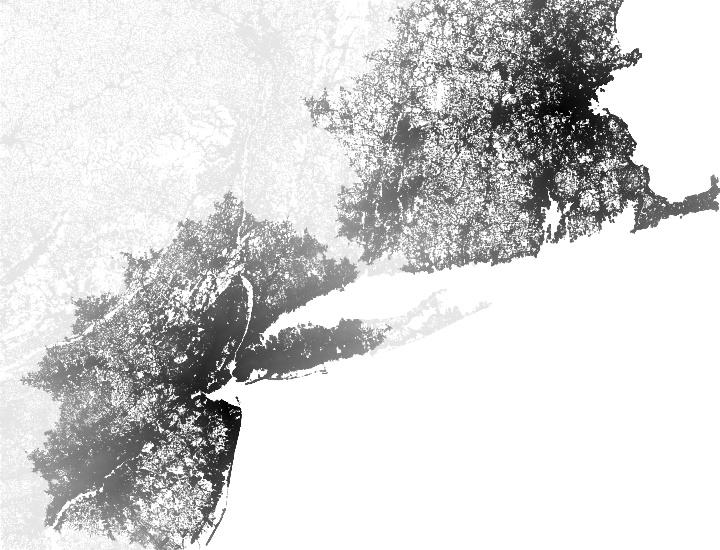
\includegraphics[width=5cm]{figs/incbi-road-ne/singleshot/example-incbi-0.png}%
   }
   
   \subfloat[Replan search]{%
      \centering%
      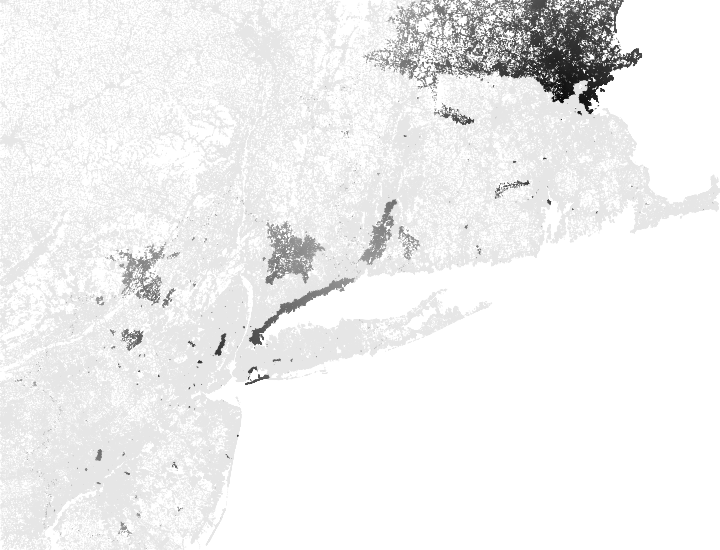
\includegraphics[width=5cm]{figs/incbi-road-ne/singleshot/example-incbi-1.png}%
   }%
   \caption{Initial search: 1,181,616 expansions.
      Replan: 262,422 expansions.}%
   \label{fig:ibid:example-incremental-bidirectional}%
\end{marginfigure}

\subsection{Bidirectional Termination with Incremental Distance Functions}

Consider a graph endowed with two distance functions,
a start distance approximation $d_s$,
and a destination distance approximation $d_t$.
Since this is an incremental setting,
we can make use of the formulation
of Theorem~\ref{thm:ibid-dynamicswsffp-sound}
from Section~\ref{sec:ibid:incremental}
to establish the correctness of these approximations
for certain vertices.

It is essential that the bidirectional termination condition from
Theorem~\ref{thm:ibid-bidir-sound} be adapted to
handle these incrementally maintained distance functions.
The central theorem that enables the IBiD algorithm is:

\begin{theorem}
Consider a graph with $w > 0$ and with $s \neq t$.
Consider a start distance approximation $d_s: V \rightarrow \mathbb{R}$,
with $r_s$ satisfying (\ref{eqn:ibid-inc-props-rvalue}),
and let $K_s$ be the smallest value $k_s(v)$
among all inconsistent vertices,
or $\infty$ if no such vertices exist;
likewise, consider the same for a destination distance approximation
$d_t$ and its accompanying $r_t$ and $K_t$.

Define $E_{\ms{conn}}$ as the set of all edges $e_{uv}$ such that
$u$ is $s$-consistent with $d_s(u) \leq K_s$
and $v$ is $t$-consistent with $d_t(v) \leq K_t$,
and define $\ell_e$ s.t. $\ell_e(e_{uv}) = d_s(u) + w(e_{uv}) + d_t(v)$.
If $E_{\ms{conn}}$ is non-empty,
and $e^*_{uv}$ minimizes $\ell_e$
among $E_{\ms{conn}}$ with $\ell_e(e^*_{uv}) \leq K_s + K_t$,
then $\ell_e(e^*_{uv})$ is the length of the shortest path,
and $e^*_{uv}$ lies on one such path.
\label{thm:ibid-sound}
\end{theorem}

\subsection{Algorithm Design}

\paragraph{Simultaneous Incremental Searches.}
The IBiD algorithm runs two independent conventional
DynamicSWSF-FP \citep{ramalingam1996dynamicswsffp}
searches simultaneously,
one from the start vertex $s$
and one from the destination vertex $t$,
with each maintaining a separate priority queue of
inconsistent vertices $Q_s$ and $Q_t$ respectively
(Algorithm~\ref{alg:ibid-two-dynamicswsffps}).

As with a convential bidirectional search,
the two sides can be alternated arbitrarily,
except that the each queue must be processed once upon initialization
so that $d_s(s) = 0$ and $d_t(t) = 0$.

{\floatevery{algorithm}{\setlength\hsize{16.85cm}}
\begin{algorithm}[t]
   \caption{As a bidirectional algorithm,
      IBiD conducts two independent DynamicSWSF-FP searches,
      one computing distance from the start vertex $s$,
      and the other computing distance to the destination vertex $t$.}
   \label{alg:ibid-two-dynamicswsffps}
   \begin{minipage}[t]{8.2cm}
      \begin{algorithmic}[1]
         \Procedure {InitializeSource} {\,\!}
            \ForAll {$v \in V$}
               \State $d_s(v) \gets \infty; \;\; r_s(v) \gets \infty$
            \EndFor
            \State $r_s(s) \gets 0$
            \State $Q_s \gets \{ s \}$
               \Comment $\mbox{ key for } v: \min\big(r_s(v),d_s(v)\big)$
            \State $\mbox{\sc ProcessSourceQueue}()$
         \EndProcedure
         \Procedure {UpdateSourceDistance} {$v$}
            \If {$v \neq s$}
               \State $r_s(v) \gets \displaystyle\min_{u \in \mbox{\scriptsize Pred}(v)}
                  \big( d_s(u) + w(u,v) \big)$
            \EndIf
            \State Ensure $v \in Q_s$ iff $d_s(v) \neq r_s(v)$
         \EndProcedure
         \Procedure {ProcessSourceQueue} {\,\!}
            \State $u \gets Q_s.\mbox{Pop}()$
            \If {$r_s(u) < d_s(u)$}
                  \Comment over-consistent
               \State $d_s(u) \gets r_s(u)$
               \ForAll {$v \in \mbox{Succ}(u)$}
                  \State $\mbox{\sc UpdateSourceDistance}(v)$
               \EndFor
            \Else
                  \Comment under-consistent
               \State $d_s(u) \gets \infty$
               \ForAll {$v \in \mbox{Succ}(u) \cup u$}
                  \State $\mbox{\sc UpdateSourceDistance}(v)$
               \EndFor
            \EndIf
         \EndProcedure
         \algstore{ibid-two-dynamicswsffps}
      \end{algorithmic}
   \end{minipage}
   \quad
   \begin{minipage}[t]{8.2cm}
      \begin{algorithmic}[1]
         \algrestore{ibid-two-dynamicswsffps}
         \Procedure {InitializeTarget} {\,\!}
            \ForAll {$v \in V$}
               \State $d_t(v) \gets \infty; \;\; r_t(v) \gets \infty$
            \EndFor
            \State $r_t(t) \gets 0$
            \State $Q_t \gets \{ t \}$
               \Comment $\mbox{ key for } v: \min\big(r_t(v),d_t(v)\big)$
            \State $\mbox{\sc ProcessTargetQueue}()$
         \EndProcedure
         \Procedure {UpdateTargetDistance} {$u$}
            \If {$u \neq t$}
               \State $r_t(u) \gets \displaystyle\min_{v \in \mbox{\scriptsize Succ}(u)}
                  \big( w(u,v) + d_t(v) \big)$
            \EndIf
            \State Ensure $u \in Q_t$ iff $d_t(u) \neq r_t(u)$
         \EndProcedure
         \Procedure {ProcessTargetQueue} {\,\!}
            \State $v \gets Q_t.\mbox{Pop}()$
            \If {$r_t(v) < d_t(v)$}
                  \Comment over-consistent
               \State $d_t(v) \gets r_t(v)$
               \ForAll {$u \in \mbox{Pred}(v)$}
                  \State $\mbox{\sc UpdateTargetDistance}(u)$
               \EndFor
            \Else
                  \Comment under-consistent
               \State $d_t(v) \gets \infty$
               \ForAll {$u \in \mbox{Pred}(v) \cup v$}
                  \State $\mbox{\sc UpdateTargetDistance}(u)$
               \EndFor
            \EndIf
         \EndProcedure
      \end{algorithmic}
   \end{minipage}
\end{algorithm}
} % floatevery width adjustment

\paragraph{Remembering Connections.}
Theorem~\ref{thm:ibid-sound} has ramifications when designing
an algorithm.
In the case of bidirectional search
described in Section~\ref{sec:ibid:bidirectional},
the algorithm could take a shortcut since $D$-values always decreased,
so it was not necessary to remember older edges when better
ones were found.
In the incremental case,
where the start and destination distance functions $d_s$ and $d_t$
may both increase and decrease between episodes,
it is no longer sufficient to remember only the best connection
found so far.

We capture the central idea from Theorem~\ref{thm:ibid-sound}
in Algorithm~\ref{alg:ibid}.

\begin{algorithm}[t]
   \caption{IBiD Outline}
   \label{alg:ibid}
   \begin{algorithmic}[1]
      \Procedure {Main} {\,}
         \State $\mbox{\sc InitializeSource}(); \; \mbox{\sc InitializeTarget}()$
         \State $Q_c \gets \emptyset$
            \Comment $\mbox{ key for } (u,v): d_s(u) + w(u,v) + d_t(v)$
         \Loop
            \While {not $\mbox{\sc TerminationCondition}()$}
               \If {$Q_s.\mbox{TopKey} < Q_t.\mbox{TopKey}$}
                     \Comment prioritize arbitrarily
                  \State $\mbox{\sc ProcessSourceQueue}(u)$
               \Else
                  \State $\mbox{\sc ProcessTargetQueue}(u)$
               \EndIf
               \State Ensure $(u,v) \in Q_c$ iff
                  $u \neq Q_s$, $v \neq Q_t$, key $\neq \infty$
            \EndWhile
            \State $(u_c,v_c) \gets Q_c.\mbox{Top}$
            \State $\pi \gets
               ( \mbox{walk } d_s \mbox{ from } u_c \mbox{ to } s )
               \cup
               ( \mbox{walk } d_t \mbox{ from } v_c \mbox{ to } t )$
            \State wait for edges $(u,v) \in E_{\ms{delta}}$ with changed weights $w(u,v)$
            \State $\mbox{\sc NotifyWeightChanges}(E_{\ms{delta}})$
         \EndLoop
      \EndProcedure
      \Function {TerminationCondition} {\,}
         \State $(u_c,v_c) \gets Q_c.\mbox{TopKey}$
            \Comment return False if $Q_c$ empty
         \If {$Q_s.\mbox{TopKey} + Q_t.\mbox{TopKey} < d_s(u_c) + w(u_c,v_c) + d_t(v_c)$}
            \State \Return False
         \EndIf
         \If {$Q_s.\mbox{TopKey} < d_s(u_c)$
               \mbox{\bf or} $Q_t.\mbox{TopKey} < d_t(v_c)$}
            \State \Return False
         \EndIf
         \State \Return True
      \EndFunction
      \Procedure {NotifyWeightChanges} {$E_{\ms{delta}}$}
         \ForAll {$(u,v) \in E_{\ms{delta}}$}
            \State $\mbox{\sc UpdateSourceDistance}(v)$
            \State $\mbox{\sc UpdateTargetDistance}(u)$
         \EndFor
         \State Ensure $(u,v) \in Q_c$ iff
            $u \neq Q_s$, $v \neq Q_t$, key $\neq \infty$
      \EndProcedure
   \end{algorithmic}
\end{algorithm}



\section{Heuristic Search}
\label{sec:ibid:heuristic}

When examining how to assemble a heuristic-informed algorithm
that integrates bidirectional with incremental methods,
it's instructive to examine how these efforts have been addressed
in the past.

\paragraph{Review of Heuristic Methods.}
Heuristic methods such as the Graph Traverser
\citep{doran1966graphtraverser} were originally
applied to pathfinding problems in order to find non-optimal
solutions more economically.
These unidirectional methods proceed similarly to Dijkstra's algorithm,
but instead of prioritizing {\sc Open} vertices
based on their source distance $d_s$,
they use a target-directed heuristic function $h_t$.
Hart, Nilsson, and Raphael \citep{hart1968astar} discovered that
these approaches can be combined ($d_s + h_t$) to yield
an admissible algorithm (A*) for the shortest-path problem,
as long as $h_t$ meets certain conditions.
See Figure~\ref{fig:ibid:example-astar}.

\begin{marginfigure}%
   \centering%
   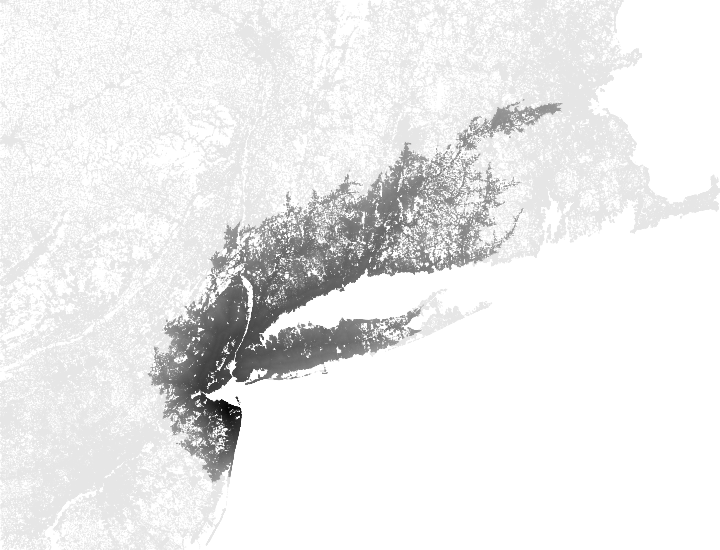
\includegraphics[width=5cm]{figs/incbi-road-ne/singleshot/example-astar.png}%
   \caption{A* search.
      532,880 expansions.}%
   \label{fig:ibid:example-astar}%
\end{marginfigure}

\subsection{Heuristic Methods in Bidirectional Search.}

Attempts to provide a bidirectional algorithm which incorporates
heuristics generally take one of three approaches.
\cdnote{I need to deep-dive here to write this correctly.}

\begin{marginfigure}%
   \centering%
   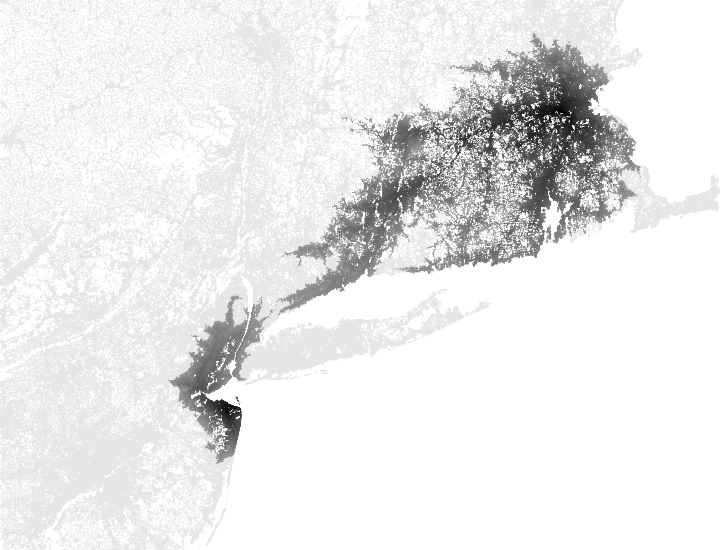
\includegraphics[width=5cm]{figs/incbi-road-ne/singleshot/example-heurbidijkstra.png}%
   \caption{Bidirectional A* search.
      515,588 expansions.}%
   \label{fig:ibid:example-heurbidijkstra}%
\end{marginfigure}
See Figure~\ref{fig:ibid:example-heurbidijkstra}.

First,
front-to-front methods
could evaluate the heuristic between all pairs in the two
{\sc Open} sets.
Expensive.

Second,
perform two heuristic-informed searches,
and account for the connection problem via a complex
termination condition.
Not necessarily efficient.
(Pohl cites Berge?)
Missile analogy.

Third,
waste (same heuristic function).

Concept of waste \citep{pohl1969bidirectional}.
I think this subsumes A*.

Talk about the 94 paper \citep{ikeda1994betterroutes}
expressing A* as a search on
the waste graph.

As a potential function.
Also Goldberg \citep{goldberg2005spexternalmemory}.

To integrate: \citep{dechter1984bfsastaropt}.

\subsection{Heuristic Methods in Incremental Search.}

Lifelong Planning A* \citep{koenig2004lpastar}.

Apply waste to incremental search to get
incremental heuristic search.

\paragraph{The Zero-Weight Problem.}
Talk about how a perfect potential leads to zero waste,
which breaks incremental search.
This motivates the lexocraphically sorted key approach.

\subsection{Heuristic IBiD}

Given a potential function which is \emph{consistent}.

Therefore all transformed edge weights are non-negative.

And with the lexographic sorting technique,
they are positive as well!

Create a transformed graph.

\paragraph{Example problem.}

For the purpose of calculating vertex heuristics,
geographic coordinates were projected onto a 2D plane using the
scale at the midpoint latitude ($41.25^\circ$)
resulting in a projecting error of less than 0.3\%.
The maximum transit speed is 30.11 m/s.

\section{Other Stuff}

\subsection{Examples}

See Figure~\ref{fig:incbi-lpastar-fig1-heurchange}
and Figure~\ref{fig:incbi-lpastar-fig1}.

\begin{figure}
   \centering%
   
   \includegraphics{build/incbi-lpastar-fig1/lpastar-heurnone-original}%
   \;\;%
   \includegraphics{build/incbi-lpastar-fig1/incbi-heurnone-original}%
   
   \vspace{0.2cm}
   
   \includegraphics{build/incbi-lpastar-fig1/lpastar-heurhalf-original}%
   \;\;%
   \includegraphics{build/incbi-lpastar-fig1/incbi-heurhalf-original}%
   
   \vspace{0.2cm}
   
   \includegraphics{build/incbi-lpastar-fig1/lpastar-heurfull-original}%
   \;\;%
   \includegraphics{build/incbi-lpastar-fig1/incbi-heurfull-original}%
   
   \caption{Illustration of behavior of IBiD on a single
      (non-incremental) shortest path problem.
      At left, IBiD uses the unidirectional start-side expansion
      strategy.
      At right, IBiD uses the bidirectional distance-balanaced
      expansion strategy.
      Start and goal heuristic functions are available;
      the unidirectional search uses a potential function based
      on the goal heuristic,
      and the bidirectional search a potential function using
      the average heuristic.
      IBiD is run with three different potential function weights:
      0.0 (top), 0.5 (middle), and 1.0 (bottom).
      IBiD therefore preforms equivalently to
      Dijkstra's algorithm (top-left),
      Bidirectional Dijkstra's (top-right),
      A* (bottom-left),
      and Bidirectional A* (bottom-right).}
   \label{fig:incbi-lpastar-fig1-heurchange}
\end{figure}

\begin{figure}
   \centering%
   
   \includegraphics{build/incbi-lpastar-fig1/lpastar-heurfull-original}%
   \;\;%
   \includegraphics{build/incbi-lpastar-fig1/lpastar-heurfull-changed}%
   
   \vspace{0.2cm}
   
   \includegraphics{build/incbi-lpastar-fig1/incbi-heurfull-original}%
   \;\;%
   \includegraphics{build/incbi-lpastar-fig1/incbi-heurfull-changed}%
   
   \caption{IBiD with only source-side expansions and a goal-side
      heuristic (top) proceeds identically to Lifelong Planning A*,
      performing 37 expansions on the original world (left)
      followed by 18 expansions over 14 vertices on the chanced
      world (right).
      IBiD with distance-balanced expansions and an average
      potential (bottom)
      performs 30 expansions on the original world
      followed by 18 expansions over 15 vertices on the changed
      world.}
   \label{fig:incbi-lpastar-fig1}
\end{figure}

\begin{figure*}
   \centering%
   
   \begin{tabular}{ccc}
      \specialcell{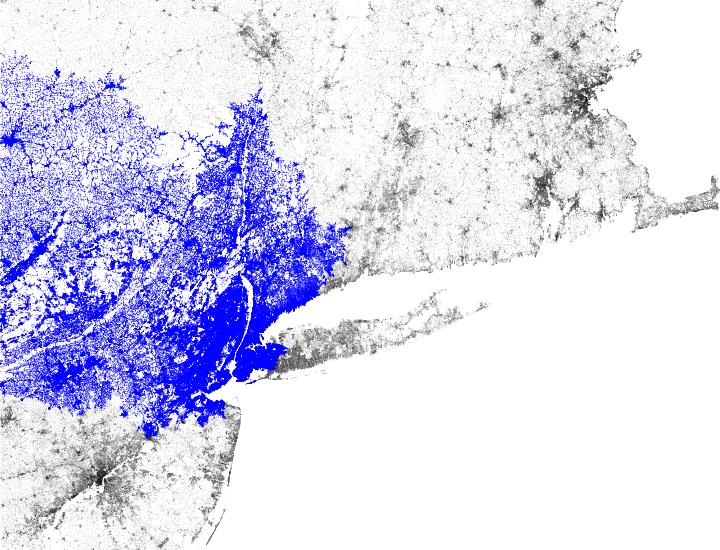
\includegraphics[width=5cm]{figs/incbi-road-ne/singleshot/pgoalnone-balfwd.png}\\556,209 expansions}
      &
      \specialcell{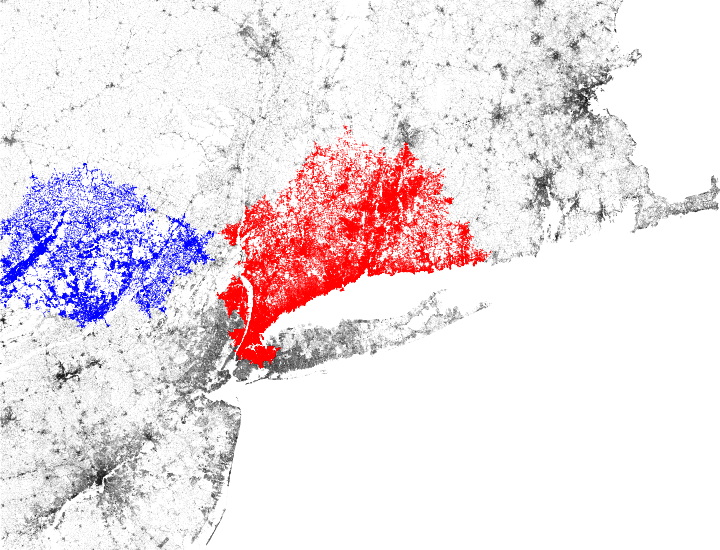
\includegraphics[width=5cm]{figs/incbi-road-ne/singleshot/pavgnone-baldist.png}\\319,938 expansions}
      &
      \specialcell{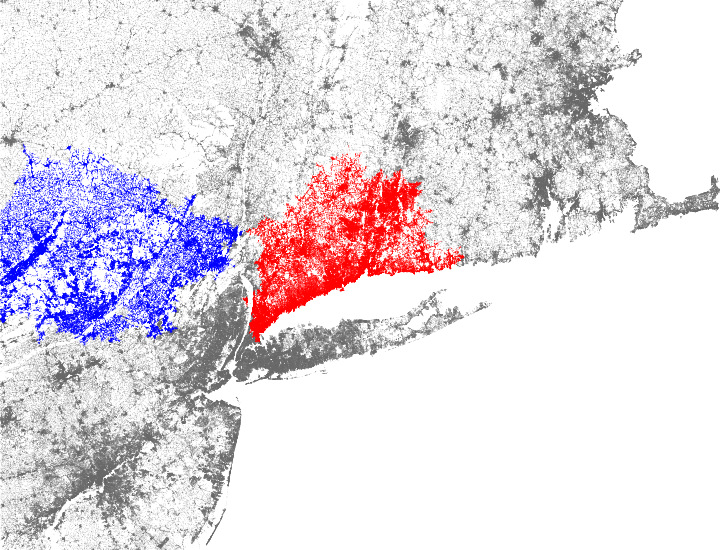
\includegraphics[width=5cm]{figs/incbi-road-ne/singleshot/pavgnone-balcard.png}\\281,413 expansions}
      \vspace{0.3cm}
      \\
      \specialcell{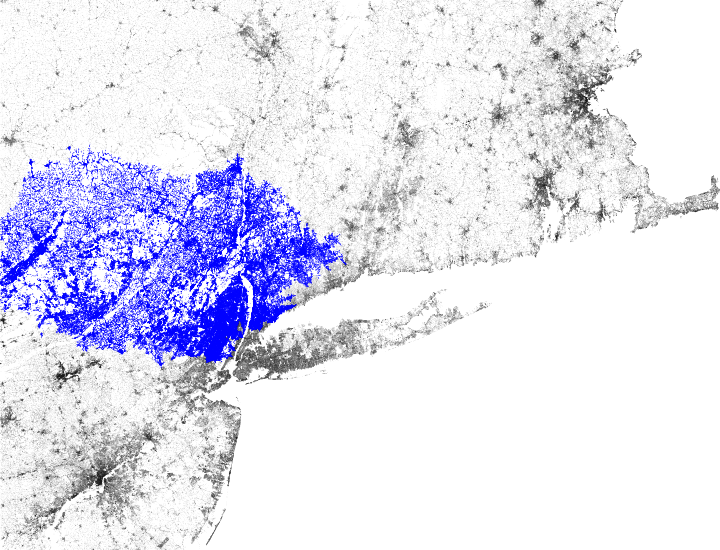
\includegraphics[width=5cm]{figs/incbi-road-ne/singleshot/pgoalhalf-balfwd.png}\\297,414 expansions}
      &
      \specialcell{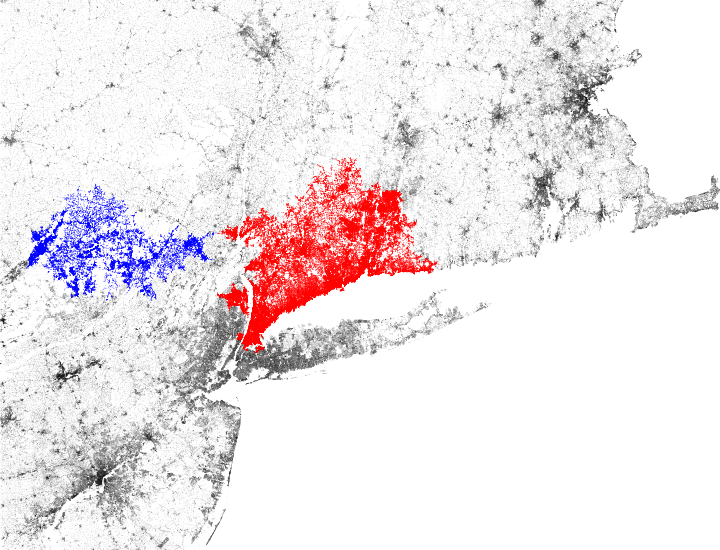
\includegraphics[width=5cm]{figs/incbi-road-ne/singleshot/pavghalf-baldist.png}\\206,625 expansions}
      &
      \specialcell{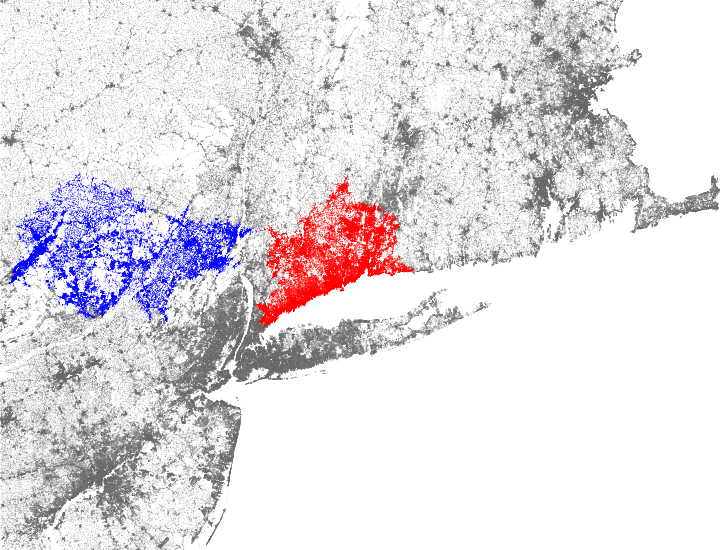
\includegraphics[width=5cm]{figs/incbi-road-ne/singleshot/pavghalf-balcard.png}\\178,929 expansions}
      \vspace{0.3cm}
      \\
      \specialcell{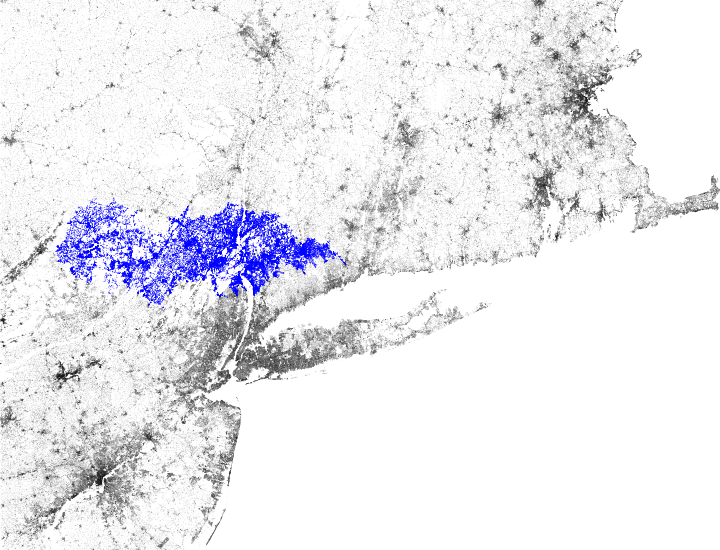
\includegraphics[width=5cm]{figs/incbi-road-ne/singleshot/pgoalfull-balfwd.png}\\82,915 expansions}
      &
      \specialcell{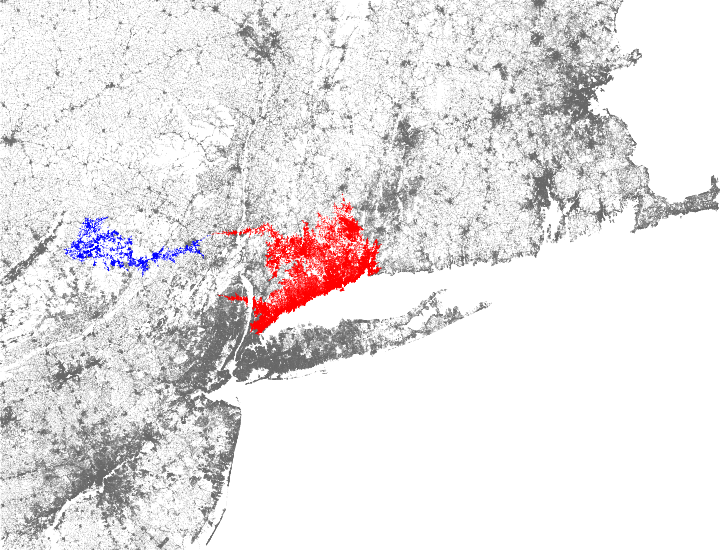
\includegraphics[width=5cm]{figs/incbi-road-ne/singleshot/pavgfull-baldist.png}\\95,759 expansions}
      &
      \specialcell{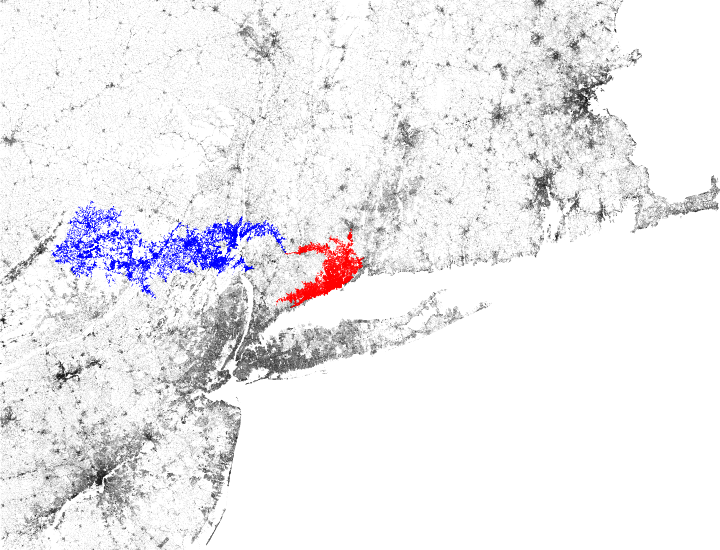
\includegraphics[width=5cm]{figs/incbi-road-ne/singleshot/pavgfull-balcard.png}\\69,218 expansions}
      \vspace{0.5cm}
   \end{tabular}
   
   \caption{Comparison between various heuristic strengths and
      balancing strageties on a single-pair road network problem.
      A path with shortest transit time is sought.
      The heuristic strength varies from no heuristic (top)
      to a full-strength heuristic (bottom).
      At left, a foward-only balancer is used, so that the
      top-left is equivalent to Dijkstra's algorithm,
      and the bottom-left is equivalent to A*.
      The middle column uses a balanced distance strategy.
      The right column uses a balanced cardinality strategy.}
   \label{fig:incbi-road-ne}
\end{figure*}



\subsection{Implementation Details}

Other implementations:
\citep{alberts1998softwaredynamicgraph}.


\section{Implications for LazySP}

Gotta talk about this stuff!

\subsection{LazySP Selector Experiments}

\begin{figure}
   \centering
   \includegraphics{build/incbi-sq/all-even}
   \caption{Across a selection of articulated robot planning instances,
      using the Even edge selector.
      Algorithms are
      \protect\tikz{\protect\node[fill=black!30,draw=black,postaction={pattern=north west lines}]{};}\;LPA*,
      \protect\tikz{\protect\node[fill=black!20,draw=black]{};}\;IBiD,
      and \protect\tikz{\protect\node[fill=black!30,draw=black,postaction={pattern=north east lines}]{};}\;Reverse LPA*.
      Results shown are cumulative search time.
      }
\end{figure}

\begin{figure}
   \centering
   \includegraphics{build/incbi-road-ne/stats}
   \caption{Road network incremental results.
      Algorithms are
      \protect\tikz{\protect\node[fill=black!30,draw=black,postaction={pattern=north west lines}]{};}\;LPA*,
      \protect\tikz{\protect\node[fill=black!20,draw=black]{};}\;IBiD,
      and \protect\tikz{\protect\node[fill=black!30,draw=black,postaction={pattern=north east lines}]{};}\;Reverse LPA*.
      }
\end{figure}

\begin{figure}
   \centering
   \includegraphics{build/incbi-sq/herbbin0}
   
   \includegraphics{build/incbi-sq/herbbin0-lambda}
   \caption{Problem: \texttt{herbbin0}.
      Lines are:
      \protect\tikz{\protect\draw[thick] (0,0) -- (0.15,0.15);} no heuristic,
      \protect\tikz{\protect\draw[densely dashed] (0,0) -- (0.15,0.15);} start heuristic,
      \protect\tikz{\protect\draw[densely dashdotted] (0,0) -- (0.15,0.15);} avg heuristic,
      \protect\tikz{\protect\draw[densely dotted] (0,0) -- (0.15,0.15);} goal heuristic.
      }
\end{figure}

\begin{figure*}
   \centering
   \includegraphics{build/incbi-sq/herbbookshelf0}
   \includegraphics{build/incbi-sq/herbbookshelf1nom}
   
   \includegraphics{build/incbi-sq/herbbookshelf0-lambda}
   \includegraphics{build/incbi-sq/herbbookshelf1nom-lambda}
   \caption{Problems: \texttt{herbbookshelf0} (left), texttt{herbbookshelf1nom} (right).}
\end{figure*}

\begin{figure*}
   \centering
   \includegraphics{build/incbi-sq/workcellef}
   \includegraphics{build/incbi-sq/workcellij}
   
   \includegraphics{build/incbi-sq/workcellef-lambda}
   \includegraphics{build/incbi-sq/workcellij-lambda}
   \caption{Problems: \texttt{workcellef} (left), \texttt{workcellij} (right).}
\end{figure*}
